%% Seminar deck: From point through density valuation to individual risk
%% assessment in the DCF method (IJFE, 2021). House style, academic register.
\documentclass[aspectratio=169,11pt]{beamer}
\usepackage{beamerthemeyc}
\usepackage{booktabs}
\renewcommand{\deckfootertitle}{Dec (2021) · From point through density valuation to individual risk assessment · IJFE}

\begin{document}

% 1 ---------------------------------------------------------------------------
\begin{frame}[plain]
  \vspace{2mm}
  {\ttfamily\scriptsize\color{ycmuted}SEMINAR DECK · YIELDCARTOGRAPHY.COM}\\[-0.3em]
  {\color{ycrule}\rule{\textwidth}{0.5pt}}
  \vspace{4mm}

  {\fontsize{19}{23}\selectfont\bfseries\color{ycink}From point through density valuation\\to individual risk assessment\\in the discounted cash flows method.\par}
  \vspace{6mm}
  {\small\bfseries Marcin Dec\par}
  {\footnotesize\color{ycmuted}Kozminski University \& FAME|GRAPE, Warsaw\par}
  \vspace{3mm}
  {\ttfamily\scriptsize\color{ycaccent}International Journal of Finance \& Economics, 26 (2021), 5621--5635 · doi:10.1002/ijfe.2084\par}
  \vfill
  \raisebox{-1mm}{
\includegraphics[height=6mm]{kozminski_logo.png}}\hspace{5mm}
  \raisebox{-1mm}{
\includegraphics[height=6mm]{grape_logo.png}}\hspace{5mm}
  \raisebox{-1mm}{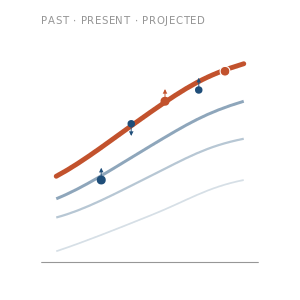
\includegraphics[height=6mm]{yc_logo.png}}
\end{frame}

% 2 ---------------------------------------------------------------------------
\begin{frame}{Motivation}
  \kicker{A point estimate conceals the uncertainty that matters}
  \begin{itemize}
    \item The discounted-cash-flow method delivers a single number,
          \( V = \sum_{t} \mathbb{E}[CF_t] \,/\, (1+r)^{t} \), from inputs
          that are themselves uncertain: projected cash flows and the
          discount rate.
    \item Sensitivity tables and scenario grids, the standard practice,
          probe the input space pointwise and carry no probability content.
          PERT (US Navy, 1958) translated qualitative scenario labels into
          numbers, but only through the first two moments under a Gaussian
          assumption.
    \item The paper reformulates the valuation to deliver the full
          distribution of outcomes implied by explicit distributions on the
          inputs, and reads risk measures off that distribution.
  \end{itemize}
\end{frame}

% 3 ---------------------------------------------------------------------------
\begin{frame}{Downside risk: the lineage}
  \kicker{From safety-first to VaR}
  \begin{itemize}
    \item Roy (1952) posits that the investor prefers safety of principal
          first, requiring a minimum acceptable return, with the
          reward-to-variability ratio as the criterion, the concept that
          evolved into the Sharpe ratio.
    \item The downside-risk literature that followed produced below-mean
          semivariance, below-target semivariance, lower partial moments,
          Value-at-Risk and VaR-equivalent volatility.
    \item Judging a simulated valuation by its first two moments alone
          wastes the model-building effort: the object of interest is the
          density, and the downside measures are functionals of it.
  \end{itemize}
\end{frame}

% 4 ---------------------------------------------------------------------------
\begin{frame}{Stochastic DCF: cash-flow decomposition}
  \kicker{Theoretical setting}
  \small Cash flows are represented by revenue, cost, scaled and fixed
  components,
  \[ CF(t) \;=\; \sum_{i=1}^{N} R_i(t) - \sum_{i=1}^{M} C_i(t)
     + \sum_{i=1}^{K} S_i\big((R_n),(C_m),(Y_e),t\big) + F, \]
  with explicit stochastic processes on the drivers and on the discount
  rate, so the valuation $V$ becomes a random variable.
  \begin{itemize}
    \item Scaled variables $S_i$ are functional forms of the directly
          simulated drivers: business-cycle-dependent prices, piecewise
          cost schedules, tax paths. They inherit randomness without their
          own SDEs.
  \end{itemize}
\end{frame}

% 5 ---------------------------------------------------------------------------
\begin{frame}{The menu of driver processes}
  \kicker{SDEs matched to sign and mean-reversion properties}
  \small For strictly signed drivers (revenues, costs):
  \[ dX_i = \mu_i X_i\,dt + \sigma_i X_i\,dW_i \;\;\text{(GBM)},
     \qquad
     dX_i = \kappa_i(\theta_i - X_i)\,dt + \sigma_i\sqrt{X_i}\,dW_i
     \;\;\text{(CIR)}. \]
  For drivers of either sign:
  \[ dX_i = \mu_i\,dt + \sigma_i\,dW_i \;\;\text{(ABM)},
     \qquad
     dX_i = \kappa_i(\theta_i - X_i)\,dt + \sigma_i\,dW_i \;\;\text{(OU)}, \]
  and for discontinuous events a pure jump process
  $dX_i = \kappa_i\,dJ_i(\lambda,t)$ with Poisson intensity $\lambda$ and
  jump magnitude $\kappa_i$. Correlation across drivers is imposed on the
  Brownian increments.
\end{frame}

% 6 ---------------------------------------------------------------------------
\begin{frame}{From simulation to density}
  \kicker{Monte Carlo, KDE and the Cornish-Fisher alternative}
  \begin{itemize}
    \item The valuation density is generated by Monte Carlo simulation of
          the driver system and estimated by kernel density methods, at both
          the cash-flow and the valuation level.
    \item A Cornish--Fisher expansion (1938) is implemented as the analytic
          alternative, capturing skewness and kurtosis beyond the Gaussian
          approximation, with the known caveats on its validity region
          (Jaschke 2002).
    \item Discrete probability mass functions remain available where the
          analyst insists on hand-shaped scenarios, at the cost of losing
          the catalogue of named-distribution properties.
  \end{itemize}
\end{frame}

% 7 ---------------------------------------------------------------------------
\begin{frame}{Individual risk assessment}
  \kicker{Functionals of the valuation density}
  \small The same density answers the pricing and the risk question:
  \begin{itemize}
    \item \textbf{Consistency check} against the risk-free benchmark
          valuation $t_{rf}$,
          \[ E \;=\; \left|\,0.5 - \tilde F_{SDCF}(t_{rf})\,\right|, \]
          which should be close to zero under the first asset-pricing
          theorem in a perfect-market limit.
    \item \textbf{Reservation valuations} at chosen confidence levels,
          \[ t_{\min,99\%} = Q(0.01,\tilde V_{SDCF}),\quad
             t_{\min,95\%} = Q(0.05,\tilde V_{SDCF}),\quad
             t_{\min,90\%} = Q(0.10,\tilde V_{SDCF}), \]
          each reader applying their own risk tolerance to one common
          object rather than a single aggregated point recommendation.
  \end{itemize}
\end{frame}

% 8 ---------------------------------------------------------------------------
\begin{frame}{Case study: correlated drivers}
  \kicker{A two-product firm over a finite horizon}
  \begin{itemize}
    \item Sales of product 1 follow GBM with $\mu_1=0.01$, $\sigma_1=0.5$,
          $X_1(0)=120$; sales of product 2 follow CIR with $\theta_2=75$,
          $\kappa_2=0.1$, $\sigma_2=0.5$, $X_2(0)=80$; a business-climate
          indicator follows OU with $\theta_3=0$, $\kappa_3=0.1$,
          $X_3(0)=5$.
    \item The three processes carry the correlation matrix with
          $\rho_{12}=0.75$, $\rho_{13}=0.1$, $\rho_{23}=-0.25$.
    \item Independent of these, surprise regulatory-adjustment costs (a
          heavily regulated market) follow a pure Poisson process with
          intensity $\lambda=0.07$, magnitude $10{,}000$ and a 50/50 sign.
  \end{itemize}
\end{frame}

% 9 ---------------------------------------------------------------------------
\begin{frame}{Case study: scaled variables}
  \kicker{Functional forms on top of the drivers}
  \begin{itemize}
    \item Prices of product 1 are business-cycle dependent: a base price of
          40 plus the business-climate indicator scaled by
          $\alpha_{P_1}=1$.
    \item Fixed costs follow a piecewise schedule in total sales $TS$:
          13{,}000 if $TS \ge 17{,}000$, 9{,}000 if $TS < 12{,}000$, and
          9{,}500 otherwise. Financial costs combine a base of 400 with a
          business-climate term scaled by $\alpha_{Int}=50$ or $-80$.
    \item The tax rate declines deterministically,
          $tax(t) = tax_{base}(1-\Delta_{tax})^{t}$, expressing a long-term
          view of falling taxes.
  \end{itemize}
\end{frame}

% 10 --------------------------------------------------------------------------
\begin{frame}{Computational performance}
  \kicker{Parsimony as a design goal}
  \begin{itemize}
    \item The exercises simulate and rescale more than 15 variables in
          300{,}000 paths within about 3 minutes on an average CPU: density
          valuation is feasible inside routine appraisal work, not only in
          dedicated risk systems.
    \item Parameters of government bond yield curves for the discount-rate
          process, frequently from the Nelson--Siegel--Svensson model, are
          freely available from central banks, which keeps recalibration
          cheap.
    \item The Cornish--Fisher route provides an even cheaper analytic
          approximation where the expansion is valid.
  \end{itemize}
\end{frame}

% 11 --------------------------------------------------------------------------
\begin{frame}{Implications}
  \kicker{For valuation practice}
  \begin{itemize}
    \item Reporting a valuation as a distribution disciplines the input
          assumptions: every scenario grid becomes a special case of an
          explicit probabilistic statement.
    \item Disagreements between valuations can be decomposed into
          disagreements about input distributions, which are auditable.
    \item Valuation and risk measurement collapse into one object, and the
          framework extends to any present-value object with uncertain
          flows and rates, from equity valuation to project finance.
  \end{itemize}
\end{frame}

% 12 --------------------------------------------------------------------------
\begin{frame}[plain]
  \vspace{12mm}
  {\fontsize{27}{31}\selectfont\bfseries\color{ycink}Thank you.\par}
  \vspace{6mm}
  {\normalsize\color{ycink}Marcin Dec\par}
  {\small\color{ycmuted}Kozminski University \& FAME|GRAPE, Warsaw\\
   mdec@kozminski.edu.pl · ORCID 0000-0002-6220-8267\par}
  \vspace{5mm}
  {\ttfamily\footnotesize\color{ycaccent}%
   Dec, M. (2021). From Point through Density Valuation to Individual\\
   Risk Assessment in the Discounted Cash Flows Method.\\
   International Journal of Finance \& Economics, 26, 5621--5635.\\
   doi:10.1002/ijfe.2084\par}
  \vfill
  \raisebox{-1mm}{
\includegraphics[height=6mm]{kozminski_logo.png}}\hspace{5mm}
  \raisebox{-1mm}{
\includegraphics[height=6mm]{grape_logo.png}}\hspace{5mm}
  \raisebox{-1mm}{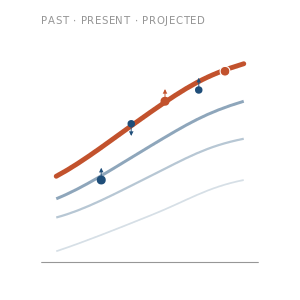
\includegraphics[height=6mm]{yc_logo.png}}
  \hfill{\ttfamily\scriptsize\color{ycmuted}yieldcartography.com/slides/dcf/}
\end{frame}

\end{document}
